\documentclass{ieeeaccess}
\usepackage{cite}
\usepackage{amsmath,amssymb,amsfonts}
\usepackage{algorithmic}
\usepackage{graphicx}
\usepackage{textcomp}
\usepackage{xcolor}

\usepackage{bm}
\makeatletter
\AtBeginDocument{\DeclareMathVersion{bold}
\SetSymbolFont{operators}{bold}{T1}{times}{b}{n}
\SetSymbolFont{NewLetters}{bold}{T1}{times}{b}{it}
\SetMathAlphabet{\mathrm}{bold}{T1}{times}{b}{n}
\SetMathAlphabet{\mathit}{bold}{T1}{times}{b}{it}
\SetMathAlphabet{\mathbf}{bold}{T1}{times}{b}{n}
\SetMathAlphabet{\mathtt}{bold}{OT1}{pcr}{b}{n}
\SetSymbolFont{symbols}{bold}{OMS}{cmsy}{b}{n}
\renewcommand\boldmath{\@nomath\boldmath\mathversion{bold}}}
\makeatother

\def\BibTeX{{\rm B\kern-.05em{\sc i\kern-.025em b}\kern-.08em
    T\kern-.1667em\lower.7ex\hbox{E}\kern-.125emX}}

% ---- Author to-do marker: renders in red so unfinished items cannot be missed. DELETE ALL BEFORE SUBMISSION. ----
\newcommand{\todo}[1]{{\color{red}\textbf{[TODO: #1]}}}
% ---- Pull in tables written by extended_experiments.py if they exist ----
\newcommand{\exttable}[2]{\IfFileExists{tables/#1.tex}{\input{tables/#1.tex}}{\par\todo{run \texttt{extended\_experiments.py} and place \texttt{\detokenize{#1}.tex} in tables/ (#2)}\par}}

\begin{document}
\history{Date of publication xxxx 00, 0000, date of current version xxxx 00, 0000.}
\doi{10.1109/ACCESS.2026.0000000}

\title{Label-Free Comparison of Outlier Detectors on 1.46 Million New York City Taxi Trip Records}
\author{\uppercase{Mehfooza M}\authorrefmark{1},
\uppercase{Likith Pulivarthi}\authorrefmark{1},
\uppercase{Rana Yash Raj Pratap Singh}\authorrefmark{1}, AND
\uppercase{Vinayak Raj}\authorrefmark{1}}

\address[1]{School of Computer Science Engineering and Information Systems (SCOPE), Vellore Institute of Technology, Vellore 632014, India}
\tfootnote{\todo{Funding/support statement, or ``This research received no external funding.''}}

\markboth
{Mehfooza \headeretal: Label-Free Comparison of Outlier Detectors on NYC Taxi Trip Records}
{Mehfooza \headeretal: Label-Free Comparison of Outlier Detectors on NYC Taxi Trip Records}

\corresp{Corresponding author: Mehfooza M (e-mail: mehfooza.m@vit.ac.in).}

\begin{abstract}
Taxi trip logs contain records that cannot describe real driving, such as multi-day durations, zero-length trips, and average speeds far beyond any legal limit. Left in place, these records distort statistical summaries and degrade predictive models, yet the choice of cleaning method is rarely justified. This paper compares four outlier detectors, the Z-score rule, Tukey's interquartile range fences, Isolation Forest, and the local outlier factor, on the 1,458,644-trip New York City Taxi Trip Duration dataset, using trip duration, great-circle distance, and average speed as features. Because the data carry no anomaly labels, we combine label-free criteria (share of trips flagged, pairwise Jaccard agreement, match against physical plausibility rules, runtime, and downstream regression error) with an injected-anomaly benchmark whose labels are known. The interquartile range rule flagged 12.51\% of trips and the Z-score rule 2.92\%. Agreement between methods was low (Jaccard 0.102 to 0.697). On raw features the local outlier factor recovered 56\% of the rule-violating trips, against 2.5\% and 4.1\% for the Z-score and interquartile range rules, but after logarithmic transformation and robust scaling the classical rules recovered all of them and the local outlier factor 28\%. On injected anomalies the interquartile range rule ranked best after scaling, and the local outlier factor ranked worst in both feature spaces. On a common test set, removing flagged trips left squared error unchanged but reduced mean absolute error by 6 to 13\%.
\end{abstract}

\begin{keywords}
Anomaly detection, data quality, interquartile range, Isolation Forest, local outlier factor, outlier detection, taxi trip data, Z-score
\end{keywords}

\titlepgskip=-21pt

\maketitle

\section{Introduction}
\label{sec:introduction}
\PARstart{M}{etered} taxis in a large city produce an enormous stream of records. Each trip carries a pickup and drop-off time, two coordinate pairs, a passenger count, and a fare, and together these records describe how a city actually moves. They are used to forecast demand, estimate travel times, plan routes, and study congestion. But the sensors that produce them operate in uncontrolled conditions: satellite signals bounce between buildings, meters are left running, and devices reboot or lose their clocks. The result is a raw log in which a few records are hundreds or thousands of times too long, too short, too fast, or too slow to be real trips.

These records matter more than their small number suggests. A single 40-day ``trip'' moves the mean duration of a million-trip dataset noticeably and can dominate any squared-error loss that is later minimized on it. Practitioners therefore clean the data before modeling, but the cleaning step is usually ad hoc: a fixed cap on duration, a speed limit chosen by eye, or a quick Z-score filter. Published taxi studies describe such steps in a sentence or two and rarely justify them against alternatives \cite{lam2015,schleibaum2022}.

The anomaly-detection literature offers many alternatives, but it is not obvious which of them suits record-level cleaning of large, heavily skewed trip data. Most taxi-specific work looks at whole trajectories, searching for detours, fraudulent routes, or unusual mobility patterns \cite{kong2024,huang2026,wang2018,eldawy2021}. General-purpose comparisons of detectors, on the other hand, use benchmark collections that are small, are often down-sampled, and do not resemble the mobility records analysts face \cite{goldstein2016,campos2016,han2022,bouman2024}. What is missing is a direct comparison, on one large real dataset, of detectors that represent distinct families: a global univariate rule, a robust univariate rule, a tree-based ensemble, and a local density method.

This paper supplies that comparison. Using the New York City Taxi Trip Duration dataset \cite{tlc2016}, which holds 1,458,644 yellow-cab trips from 2016, we derive trip distance and average speed from the raw coordinates and timestamps, and then apply the Z-score rule, Tukey's interquartile range (IQR) fences, Isolation Forest, and the local outlier factor (LOF). The dataset has no anomaly labels, which is the usual situation in practice, so we cannot report precision or recall in the classical sense. Instead we assemble five label-free criteria that look at the detectors from different directions, and we are explicit about what each one can and cannot show.

The main contributions are the following.
\begin{enumerate}
\item A record-level comparison of four detector families on a single large taxi dataset, with all four run on the same engineered feature vector of duration, distance, and speed.
\item A label-free, multi-criterion evaluation protocol (flag rate, pairwise Jaccard agreement, physical plausibility, runtime, and downstream regression error) that can be reused on any unlabeled tabular dataset.
\item Evidence that agreement between detectors and the plausibility of what they flag are different things, and that both depend strongly on feature scale: on raw features upper-fence rules cannot flag implausibly \emph{small} values and LOF recovers far more of the rule-violating trips, but after a logarithmic transformation with robust scaling the ordering reverses.
\item A sensitivity and reproducibility analysis of the two parameterized detectors, together with practical guidance on which detector to use under which operating constraint.
\end{enumerate}

This article extends our earlier conference paper \cite{conf2026}. Relative to that version we add a broader review of related work, a formal statement of the evaluation criteria, a recall analysis of the plausibility reference set, a detailed treatment of why the detectors diverge, a discussion of threats to validity, a corrected downstream-regression protocol (the conference protocol had an evaluation flaw, described in Section~\ref{sec:results}), and additional experiments covering robust and multivariate baselines, feature scaling, an injected-anomaly benchmark with known labels, two-stage pipelines, and full-dataset LOF (Section~\ref{sec:extended}).

The remainder of the paper is organized as follows. Section~\ref{sec:related} reviews related work. Section~\ref{sec:data} describes the dataset and engineered features. Section~\ref{sec:method} presents the detectors and the evaluation framework. Section~\ref{sec:setup} gives the experimental setup, Section~\ref{sec:results} reports results, Section~\ref{sec:extended} reports the extended experiments, Section~\ref{sec:discussion} discusses the findings and their limits, and Section~\ref{sec:conclusion} concludes.

\section{Related Work}
\label{sec:related}

\subsection{Surveys and benchmarks of anomaly detection}
Chandola \emph{et al.} organized the field around the assumptions that different techniques make about what ``normal'' means, and noted that a method is only as good as the fit between its assumption and the data \cite{chandola2009}. Later surveys narrowed the focus to high-dimensional numerical data \cite{zimek2012} and to deep models \cite{pang2021}. Aggarwal's monograph and Hawkins's earlier definition of an outlier as an observation that arouses suspicion of a different generating mechanism remain standard references for the terminology we use here \cite{hawkins1980,aggarwal2017}.

Empirical comparisons have repeatedly found that no detector wins everywhere. Goldstein and Uchida evaluated 19 unsupervised algorithms on 10 datasets and examined, among other things, how global and local anomaly behavior affects the results \cite{goldstein2016}. Campos \emph{et al.} studied neighborhood-based methods across a wide range of datasets and questioned how suitable common benchmark datasets and evaluation measures are for outlier detection \cite{campos2016}. ADBench extended the exercise to 30 algorithms on 57 datasets and concluded that algorithm selection for unsupervised problems is task dependent \cite{han2022}. Bouman \emph{et al.} compared 33 algorithms on 52 tabular datasets and reported that an extended Isolation Forest did best on ``global'' datasets and a nearest-neighbor method on ``local'' ones \cite{bouman2024}. These studies are the closest methodological relatives of our work. They differ from it in two respects: their datasets are modest in size and come with labels, and none of them is a record-cleaning study on mobility data, where the practical question is not ranking quality but which records to discard.

\subsection{Statistical and robust methods}
The Z-score rule flags observations several standard deviations from the mean and is among the most widely used baselines \cite{agarwal2021}. Its weakness is well known: both the mean and the standard deviation are themselves inflated by the outliers the rule is meant to find \cite{leys2013,rousseeuw2011}. Tukey's fences replace them with quartiles and are therefore less affected \cite{tukey1977}. Leys \emph{et al.} advocate the median absolute deviation (MAD) as a still more robust scale estimate \cite{leys2013}, and Iglewicz and Hoaglin proposed a modified Z-score built on it \cite{iglewicz1993}. For multivariate data, robust covariance estimators such as the minimum covariance determinant \cite{rousseeuw1999} give Mahalanobis distances that resist contamination. Data-quality frameworks for large structured data have adopted percentile-based rules for exactly these reasons \cite{widad2023}.

\subsection{Density-based and isolation-based methods}
Breunig \emph{et al.} introduced the local outlier factor, which compares the density around a point with the densities around its neighbors \cite{breunig2000}. Because the comparison is local, LOF can find points that are unremarkable globally but sparse relative to their surroundings; Schubert \emph{et al.} later generalized the notion of locality \cite{schubert2014}. Density reasoning has transferred to other moving-object domains, for instance to vessel trajectories \cite{zhang2023ships}. Isolation Forest takes the opposite view and builds random trees in which anomalies, being few and different, are isolated after fewer splits \cite{liu2008}. Its training cost depends on the subsample size rather than on the dataset size, which is why it scales to large inputs. Hariri \emph{et al.} identified score artifacts caused by axis-parallel splits and proposed random-hyperplane cuts \cite{hariri2021}. Open-source toolkits now make these detectors routine to apply \cite{pedregosa2011,zhao2019pyod}.

\subsection{Trajectory and taxi-specific anomaly detection}
Zheng's survey places outlier detection within the wider pipeline of trajectory mining and treats data cleaning as a separate preprocessing stage \cite{zheng2015}. Work on taxis proper concentrates on trajectory-level or route-level anomalies: taxonomies of mobile-trajectory anomaly detection \cite{kong2024}, multi-sector representations for abnormal segments \cite{huang2026}, flow embeddings that avoid hand-written rules \cite{frantzen2021}, edit-distance clustering of taxi routes \cite{wang2018}, and real-time detection of fraudulent drivers \cite{eldawy2021}. Trip-level studies address abnormal demand patterns \cite{markou2017} and duration prediction on the same TLC data we use \cite{poongodi2022}. Duration-prediction work typically handles dirty records with fixed rules. Lam \emph{et al.}, working on Porto taxi trips, flagged gross GPS errors by comparing implied speed with a plausible maximum \cite{lam2015}, and Schleibaum \emph{et al.} removed New York trips with implausible duration, distance, or location before training an ensemble \cite{schleibaum2022}. Such rules work, but their thresholds are chosen by the analyst, and the papers do not compare them with statistical or learned detectors.

\subsection{Research gap}
To our knowledge, no earlier study compares a global univariate rule, a robust univariate rule, an isolation ensemble, and a local density method for \emph{record-level} cleaning of a large taxi trip dataset, using a protocol that does not depend on labels and that reports agreement, plausibility, cost, and downstream effect together. The present work addresses that gap.

\section{Dataset and Feature Engineering}
\label{sec:data}

\subsection{Source}
We use the training partition of the New York City Taxi Trip Duration dataset, originally released by the New York City Taxi and Limousine Commission and distributed through Kaggle \cite{tlc2016}. It contains 1,458,644 yellow-cab trips recorded in 2016. Every record has a trip identifier, a vendor identifier, pickup and drop-off timestamps, a passenger count, pickup and drop-off longitude and latitude, a store-and-forward flag, and the trip duration in seconds.

\subsection{Engineered features}
Outlier detection here is unsupervised, so trip duration is treated as one component of the feature vector rather than as a prediction target. Two further quantities are derived from the raw fields. Trip distance is the great-circle distance between the pickup and drop-off coordinates, computed with the haversine formula \cite{sinnott1984}, and average speed follows from distance and duration:
\begin{equation}
v = \frac{d}{t/3600},
\label{eq:speed}
\end{equation}
where $d$ is the trip distance in kilometers, $t$ is the duration in seconds, and $v$ is the speed in km/h. Each trip is then described by $\mathbf{x}=(t,\,d,\,v)$. Two caveats follow from this construction. First, $v$ is a deterministic function of $t$ and $d$, so the three features are not independent; the speed feature is useful because it exposes combinations of $t$ and $d$ that are individually plausible but jointly impossible. Second, $d$ is a straight-line distance and therefore underestimates the driven distance, so $v$ is a lower bound on the true speed.

\subsection{Evidence of data-quality problems}
Basic profiling confirms that the dataset is a sensible testbed. Durations range from one second to several days, which is incompatible with normal taxi operation. Distances include exact zeros as well as a few trips beyond 300~km, which is not possible for an intra-city fare. Most average speeds are below 20~km/h, but a few records exceed 120~km/h. A handful of pickup or drop-off coordinates fall outside the New York metropolitan area, some of them in open water, which is consistent with GPS logging faults (Fig.~\ref{fig:scatter-loc}). A small number of records also report more than six passengers, more than a New York taxi may carry. The engineered features have no missing values. Table~\ref{tab:desc} summarizes the distributions. The gap between mean and median, and the size of the maxima relative to the standard deviations, show how strongly right-skewed all three quantities are.

\begin{table}[!t]
\caption{Descriptive statistics of the dataset (1,458,644 records).}
\label{tab:desc}
\centering
\setlength{\tabcolsep}{3pt}
\small
\begin{tabular}{lccccc}
\hline
Variable & Mean & Std. dev. & Min & Max & Median \\
\hline
Duration (s) & 959.49 & 5237.43 & 1.0 & $3.52\times10^{6}$ & 662.00 \\
Distance (km) & 3.44 & 4.29 & 0.0 & $1.24\times10^{3}$ & 2.09 \\
Speed (km/h) & 14.42 & 14.97 & 0.0 & $9.27\times10^{3}$ & 12.79 \\
Passengers & 1.66 & 1.31 & 0.0 & $9.0$ & 1.00 \\
\hline
\end{tabular}
\end{table}

Figure~\ref{fig:hist} shows the duration distribution on a logarithmic scale. Even there a thin tail of extreme values is visible to the right of the main mass. The correlation matrix in Fig.~\ref{fig:corr} shows only weak linear association between duration and distance (0.09), a low figure that is consistent with contamination, since a few extreme records can dominate a product-moment correlation.

\begin{figure}[!t]
\centering
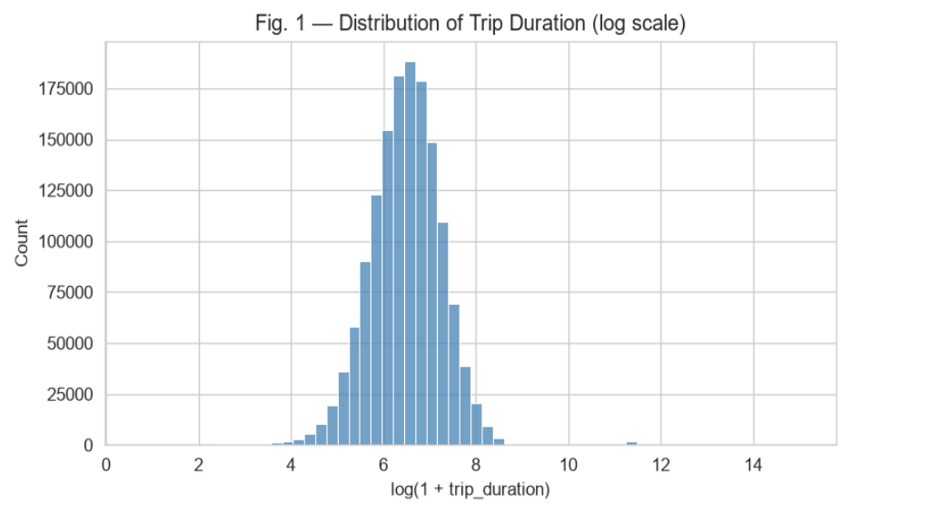
\includegraphics[width=\columnwidth]{mehfo1.png}
\caption{Histogram of trip duration on a logarithmic scale.}
\label{fig:hist}
\end{figure}

\begin{figure}[!t]
\centering
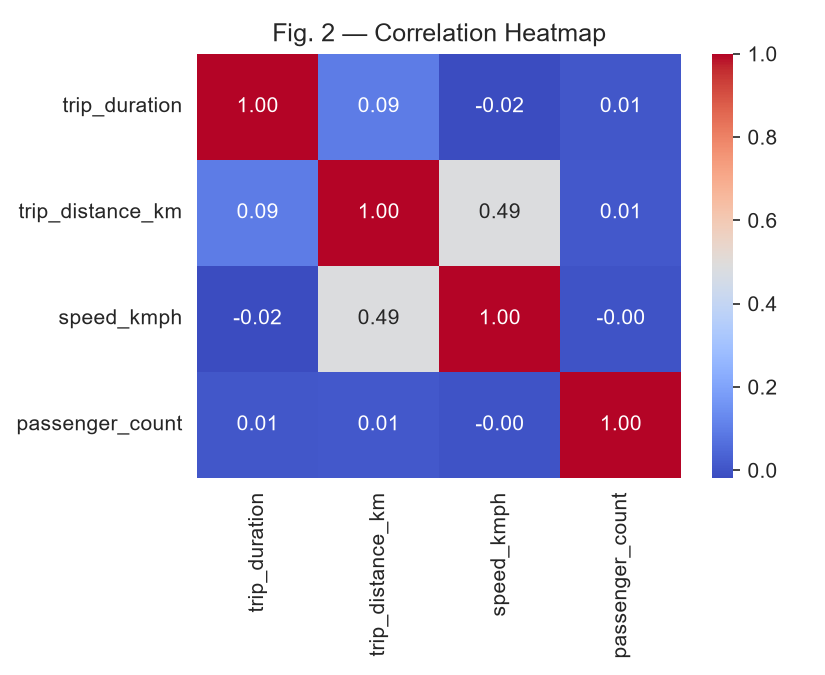
\includegraphics[width=0.85\columnwidth]{mehfo2.png}
\caption{Pearson correlation among trip duration, distance, speed, and passenger count.}
\label{fig:corr}
\end{figure}

\begin{figure}[!t]
\centering
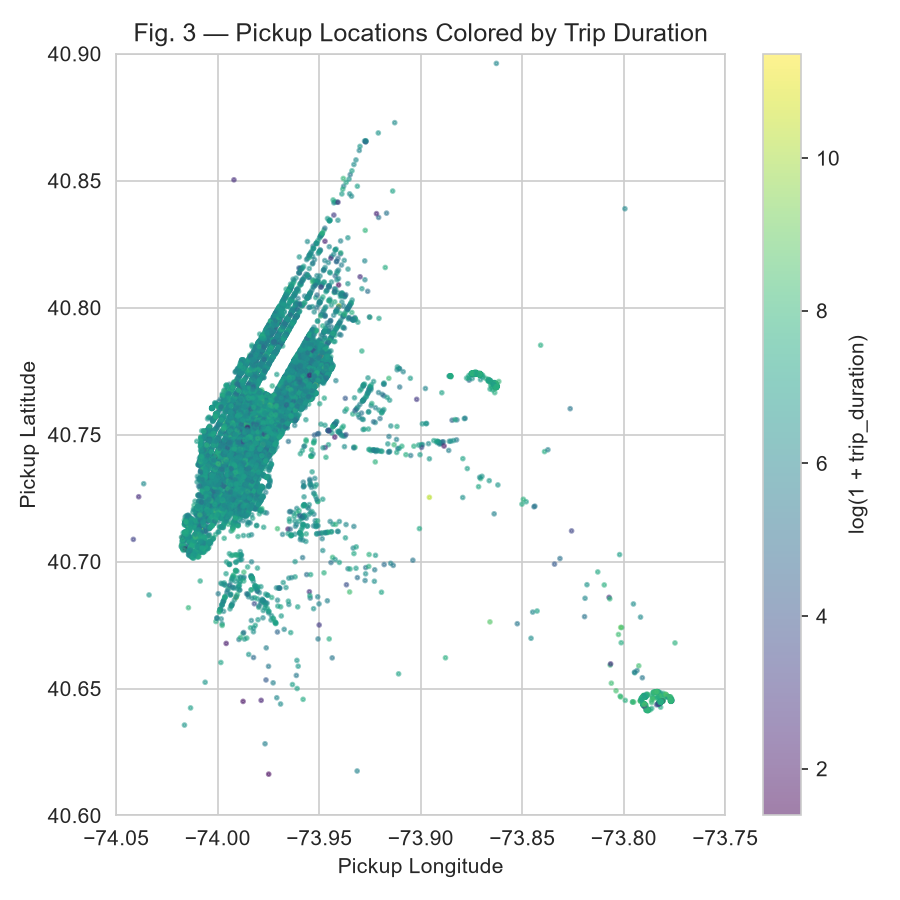
\includegraphics[width=0.85\columnwidth]{mehfo3.png}
\caption{Pickup locations colored by log trip duration. A few points lie far outside the expected service area.}
\label{fig:scatter-loc}
\end{figure}

\subsection{Preprocessing}
Fields are type-checked and the timestamps parsed before features are engineered. Records with zero duration would make (\ref{eq:speed}) undefined and are removed by a filter for non-finite values, applied before any profiling or detection. In this dataset the filter removed no records (Table~\ref{tab:ext_setup}), because the shortest recorded duration is one second. Records with zero distance but nonzero duration give a valid speed of zero and are \emph{kept}. A fare that starts and ends at the same place is itself a plausible kind of anomaly, so such records stay eligible to be flagged by any detector rather than being excluded in advance.  The base experiments apply no feature scaling: Z-score, IQR, and Isolation Forest are scale-invariant in the sense that they treat each feature separately or split on raw values, and LOF was run on raw features as in common practice. Section~\ref{sec:extended} revisits this choice, because Euclidean neighbor distances are \emph{not} scale invariant.

\section{Methodology}
\label{sec:method}

\subsection{Problem formulation}
Each trip is represented by $\mathbf{x}=(t,d,v)$. A detector is a function $f:\mathbf{x}\mapsto\{0,1\}$, with $1$ meaning the trip is flagged. No ground-truth labels exist, so the aim is to characterize and compare the detectors' behavior rather than to estimate absolute accuracy.

\subsection{Z-score rule}
For a feature value $x$ with mean $\mu$ and standard deviation $\sigma$,
\begin{equation}
z=\frac{x-\mu}{\sigma}.
\end{equation}
A trip is flagged if $|z|>3$ for any of the three features. The threshold of three is a common convention that balances sensitivity against false alarms when the data are roughly normal \cite{agarwal2021}. The mean and standard deviation are estimated on the full, unfiltered data. This is inherent to the rule: estimating them on already-cleaned data would require the outcome of the cleaning in advance.

\subsection{Interquartile range rule}
Let $Q_1$ and $Q_3$ be the 25th and 75th percentiles of a feature and $\mathrm{IQR}=Q_3-Q_1$. A trip is flagged if any feature satisfies
\begin{equation}
x<Q_1-1.5\,\mathrm{IQR}\quad\text{or}\quad x>Q_3+1.5\,\mathrm{IQR}.
\end{equation}
These are Tukey's fences \cite{tukey1977}. Quartiles are far less affected by extreme values than the mean and standard deviation, which makes the rule better suited to skewed variables such as duration and speed.

\subsection{Isolation Forest}
Isolation Forest grows $\tau$ random binary trees, each built by repeatedly choosing a feature and a split value at random until every point in its subsample is isolated. The anomaly score of a point $\mathbf{x}$ is
\begin{equation}
s(\mathbf{x},n)=2^{-\mathbb{E}[h(\mathbf{x})]/c(n)},
\end{equation}
where $h(\mathbf{x})$ is the path length from the root to the leaf containing $\mathbf{x}$, $\mathbb{E}[h(\mathbf{x})]$ is its average over trees, and $c(n)=2H(n-1)-2(n-1)/n$ is the average path length of an unsuccessful search in a binary search tree of $n$ points, with $H(i)$ the harmonic number \cite{liu2008}. Scores near one mean short average paths and a high likelihood of being anomalous. We flag the trips whose scores fall in the top fraction given by the contamination parameter, set to 0.05.

\subsection{Local outlier factor}
For a point $A$ with $k$ nearest neighbors $N_k(A)$, the reachability distance to a neighbor $B$ is
\begin{equation}
\operatorname{reach\text{-}dist}_k(A,B)=\max\{k\text{-distance}(B),\,d(A,B)\}.
\end{equation}
The local reachability density is the inverse of the mean reachability distance to the neighbors,
\begin{equation}
\operatorname{lrd}_k(A)=\left(\frac{\sum_{B\in N_k(A)}\operatorname{reach\text{-}dist}_k(A,B)}{|N_k(A)|}\right)^{-1},
\end{equation}
and the LOF score is the average ratio of the neighbors' densities to that of $A$,
\begin{equation}
\operatorname{LOF}_k(A)=\frac{1}{|N_k(A)|}\sum_{B\in N_k(A)}\frac{\operatorname{lrd}_k(B)}{\operatorname{lrd}_k(A)}.
\end{equation}
A score near one means the point is about as dense as its neighborhood; a score well above one means it is sparser than its neighbors \cite{breunig2000}. We use $k=20$ and the same 0.05 contamination as for Isolation Forest, so that the two are comparable.

\subsection{Evaluation framework}
Without labels, none of the criteria below measures true precision or recall. Each gives comparative evidence about one aspect of behavior.

\emph{(i) Flag rate.} The fraction of trips each detector flags.

\emph{(ii) Agreement.} For flagged sets $A$ and $B$, the Jaccard similarity is
\begin{equation}
J(A,B)=\frac{|A\cap B|}{|A\cup B|}.
\end{equation}
A low value means that the detectors disagree about \emph{which} trips are unusual, not merely about how many.

\emph{(iii) Physical plausibility.} A fixed reference set $R$ is built from three rules applied directly to the raw feature values, before any detector runs: speed above 120~km/h, duration below 10~s, or distance below 0.01~km. For a detector that flags set $F$ we report
\begin{equation}
\mathrm{Prec}=\frac{|F\cap R|}{|F|},\qquad \mathrm{Rec}=\frac{|F\cap R|}{|R|}.
\end{equation}
Precision is the share of flags that violate a rule; recall is the share of rule violators the detector found. The thresholds are reasoned rather than data-derived: 120~km/h is well above any posted limit on New York roads, ten seconds is shorter than any plausible pickup-to-drop-off cycle, and ten meters is below the positional accuracy of consumer GPS receivers. They are nevertheless arbitrary, and $R$ is a proxy for implausibility, not ground truth.

\emph{(iv) Runtime.} Wall-clock time of each detector.

\emph{(v) Downstream effect.} A linear regression predicts duration from trip distance, passenger count, pickup hour, and pickup day of week. For each of several random 80/20 splits of the development sample, every detector is fitted on the training partition only, its flagged training trips are removed, and the regression is fitted on what remains. Every regression, whatever its detector, is then scored on the \emph{same} held-out partition, both as it stands and after removing trips that violate the plausibility rules. We report RMSE together with mean absolute error, median absolute error, and root-mean-square logarithmic error, because RMSE alone is dominated by a few extreme targets. Speed is deliberately not a predictor: it is computed from the duration being predicted.

\section{Experimental Setup}
\label{sec:setup}
Table~\ref{tab:hyper} lists the hyperparameters. The 5\% contamination used for Isolation Forest and LOF was not tuned. It was set well above the 0.68\% of development-sample records (676 of 100,000) that violate at least one plausibility rule, so that borderline records that are statistically extreme without breaking a hard rule, such as an unusually slow or long trip, can also be captured. Because both detectors flag exactly the requested fraction, their flag rates reflect this choice rather than the data, and all conclusions about them are conditional on it. Section~\ref{sec:results} shows how flagged counts scale with the parameter. All computation was done in Python with pandas, NumPy, SciPy, and scikit-learn \cite{pedregosa2011}, and the figures with matplotlib and seaborn. Table~\ref{tab:ext_setup} records the data counts, software versions, and the machine used for the experiments in Section~\ref{sec:extended}. The runtimes in Tables~\ref{tab:dev} and~\ref{tab:full} come from the conference-version runs and are used only to compare detectors within each table. \todo{State the hardware (CPU, cores, RAM) used for Tables~\ref{tab:dev} and~\ref{tab:full}, or replace the timings in those tables with ones from your own rerun of run\_all.py.}

\exttable{ext_setup}{Table: data counts and computing environment}

\begin{table}[!t]
\caption{Detector hyperparameters.}
\label{tab:hyper}
\centering
\small
\begin{tabular}{ll}
\hline
Detector & Settings \\
\hline
Z-score & threshold $=3\sigma$, any of three features \\
IQR & $1.5\times$IQR (Tukey's fences), any of three features \\
Isolation Forest & contamination $=0.05$, seed $=42$ \\
LOF & $k=20$, contamination $=0.05$ \\
\hline
\end{tabular}
\end{table}

The outlier-detection step itself is unsupervised and needs no train/test split. The 80/20 split is used only for the downstream regression evaluation.

\section{Results}
\label{sec:results}

\subsection{Flag rates and runtime}
Table~\ref{tab:dev} gives the results on the 100,000-row development sample, and Table~\ref{tab:full} gives the full-dataset results. Unless stated otherwise, the percentages and runtimes discussed below are the full-dataset figures.

\begin{table}[!t]
\caption{Detection results on the 100,000-row development sample.}
\label{tab:dev}
\centering
\small
\begin{tabular}{lccc}
\hline
Technique & Flagged (\%) & Count & Runtime (s) \\
\hline
Z-score & 3.602 & 3602 & 0.020 \\
IQR & 12.525 & 12525 & 0.026 \\
Isolation Forest & 4.999 & 4999 & 1.568 \\
LOF & 5.000 & 5000 & 0.530 \\
\hline
\end{tabular}
\end{table}

\begin{table}[!t]
\caption{Detection results on the full dataset. LOF was run on a 300,000-row sub-sample and is not directly comparable to the other rows.}
\label{tab:full}
\centering
\small
\begin{tabular}{lccc}
\hline
Technique & Rows used & Flagged (\%) & Runtime (s) \\
\hline
Z-score & 1,458,644 & 2.922 & 0.160 \\
IQR & 1,458,644 & 12.514 & 0.200 \\
Isolation Forest & 1,458,644 & 5.000 & 18.552 \\
LOF (sub-sample) & 300,000 & 5.000 & 1.673 \\
\hline
\end{tabular}
\end{table}

The IQR rule flagged more than four times as many trips as the Z-score rule (12.51\% against 2.92\%). Both rules operate on the same three variables, so the difference comes from how each defines the acceptable range. Duration and speed are strongly right-skewed (Fig.~\ref{fig:hist}), and the few extreme records inflate the standard deviation that the Z-score threshold is built on. With $\sigma$ already large, three standard deviations reach far into the tail and the rule tolerates a great many moderately unusual trips. Quartiles are barely moved by a handful of extreme values, so the IQR fences stay close to the bulk of the data and catch more of the upper tail. This is consistent with the Z-score rule's drop from 3.60\% on the development sample to 2.92\% on the full data, where the more extreme records of the larger file can stretch the standard deviation further. By contrast, the IQR rate is almost unchanged (12.53\% to 12.51\%).

LOF was run on 300,000 rows only, one fifth of the data, so its flag rate and runtime in Table~\ref{tab:full} are sample-specific. Agreement and plausibility comparisons (Tables~\ref{tab:jaccard} and~\ref{tab:plaus}) are therefore computed on the shared development sample, where all four detectors see the same trips. Section~\ref{sec:extended} reports a full-dataset LOF run that removes this caveat.

\subsection{Inter-method agreement}
Table~\ref{tab:jaccard} and Fig.~\ref{fig:jaccard} report pairwise Jaccard similarity. Isolation Forest and the Z-score rule overlap strongly ($J=0.697$): both are driven by extreme magnitudes, and the trips that sit far from the bulk of the distribution are caught by both. Every other pair overlaps weakly. The IQR rule and Isolation Forest reach 0.379, the IQR and Z-score rules 0.288, and LOF shares little with anyone (0.102 to 0.120). Four detectors that all claim to find ``unusual'' trips are in practice flagging largely different sets. Choosing one of them is therefore a substantive modeling decision.

\begin{table}[!t]
\caption{Jaccard similarity between flagged sets (development sample).}
\label{tab:jaccard}
\centering
\small
\setlength{\tabcolsep}{3pt}
\begin{tabular}{lcccc}
\hline
Method & Z-score & IQR & Isol. Forest & LOF \\
\hline
Z-score & 1.000 & 0.288 & 0.697 & 0.102 \\
IQR & 0.288 & 1.000 & 0.379 & 0.115 \\
Isolation Forest & 0.697 & 0.379 & 1.000 & 0.120 \\
LOF & 0.102 & 0.115 & 0.120 & 1.000 \\
\hline
\end{tabular}
\end{table}

\begin{figure}[!t]
\centering
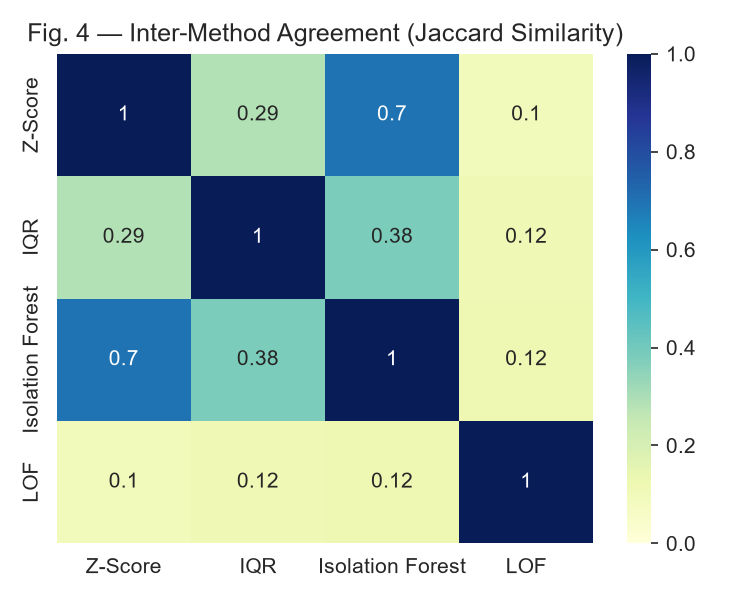
\includegraphics[width=0.9\columnwidth]{mehfo4.png}
\caption{Pairwise Jaccard similarity between the sets of trips flagged by each detector.}
\label{fig:jaccard}
\end{figure}

\subsection{Physical plausibility}
The reference set $R$ contains 676 of the 100,000 development-sample trips. It was fixed before any detector was run, so it does not depend on the output being evaluated. Table~\ref{tab:plaus} reports the precision values obtained in our experiments together with the number of rule-violating trips each detector found and the recall. Hits are the number of flagged trips that fall in $R$, and recall is hits divided by $|R|=676$.

\begin{table}[!t]
\caption{Overlap of each detector's flags with the plausibility reference set $R$ ($|R|=676$). Hits and recall are computed from the same run as the precision values.}
\label{tab:plaus}
\centering
\small
\setlength{\tabcolsep}{3pt}
\begin{tabular}{lccc}
\hline
Technique & Precision (\%) & Hits in $R$ & Recall (\%) \\
\hline
Z-score & 0.472 & 17 & 2.5 \\
IQR & 0.224 & 28 & 4.1 \\
Isolation Forest & 4.041 & 202 & 29.9 \\
LOF & 7.600 & 380 & 56.2 \\
\hline
\end{tabular}
\end{table}

LOF achieved the highest precision (7.60\%), nearly twice that of Isolation Forest and more than fifteen times that of either classical rule. The recall shows the same ordering, with LOF recovering 380 of the 676 rule-violating trips. The two classical rules found only 17 and 28. Even LOF's precision is low in absolute terms, which is expected: 5\% of the data is flagged while only 0.68\% breaks a rule, so even a perfect detector at this contamination would score no more than 13.5\% precision. Read this way, LOF's 7.6\% is more than half of the attainable maximum.

The very low recall of the Z-score and IQR rules has a simple explanation. The reference set consists mostly of trips that are \emph{too short} or cover \emph{too little distance}. Speeds above 120~km/h are rare, and the Z-score and IQR rules flag them reliably, so at most 17 of the 676 trips can be speed violators. That leaves roughly 650 or more records with a duration below ten seconds or a distance below ten meters. Those are small-value anomalies, and an upper-fence rule on a positive, right-skewed variable may have no usable lower fence at all. Table~\ref{tab:ext_fences} shows that this is the case here: the lower boundaries of both rules are negative for all three features (for the IQR rule, $-629.5$~s, $-2.73$~km, and $-3.97$~km/h), so neither rule can flag a too-short duration, a too-small distance, or a too-low speed.

\exttable{ext_fences}{Table: lower and upper boundaries of the Z-score and IQR rules}

LOF, which measures sparsity in both directions, is not subject to this blind spot. Section~\ref{sec:extended} shows, however, that the ordering depends on feature scale and reverses after a logarithmic transformation.

\subsection{Downstream regression impact}
The conference version of this study reported that removing IQR-flagged trips lowered regression RMSE from 3199.69 to 289.07 s, far more than removing LOF-flagged trips (3036.70 s). Table~\ref{tab:ext_protocol} reproduces those values exactly. On re-examining the protocol we found that it does not support comparisons between detectors. The whole 100,000-row sample was cleaned \emph{before} the 80/20 split, so each detector's regression was scored on a different, filtered test set, and the detectors had seen the test trips when they were fitted. Removing the extreme trips from the test set removes most of the squared error, which is the most plausible reason the Z-score, IQR, and Isolation Forest rows fall so far; the drop reflects the deletion of extreme test targets rather than a better model, as the corrected protocol below confirms.

\exttable{ext_protocol}{Table: RMSE under the conference-version protocol}

Under the corrected protocol of Section~\ref{sec:method} (detectors fitted on the training partition only, one common held-out set, several random splits), RMSE is essentially the same for every condition, including no cleaning at all: all values lie between about 3245 and 3267 s, with a standard deviation of roughly 240 s across splits (Table~\ref{tab:ext_downstream}). A few extreme test targets dominate squared error, and a linear model fitted on any version of the training data cannot predict them. The absolute-error measures do respond. In the raw feature space, mean absolute error falls from 472.7~s without cleaning to between 412.3~s (Isolation Forest) and 443.9~s (LOF), a reduction of 6 to 13\%, and median absolute error falls from 312.7~s to between 197.2~s (IQR) and 264.6~s (LOF). The differences among the IQR, Z-score, and Isolation Forest rules in mean absolute error (412 to 425~s) are about the size of the split-to-split standard deviation (about 20~s) and should not be over-interpreted; LOF's smaller improvement is clearer. The same ordering holds on the rule-clean partition.

\subsection{Sensitivity analysis}
Figure~\ref{fig:sens} shows how flagged counts respond to the detector parameters. The number of trips flagged by Isolation Forest grows linearly with the contamination setting, from about 1,000 at 0.01 to 5,000 at 0.05 and 10,000 at 0.10, which confirms that the setting, not the data, determines the flag rate. LOF's flagged count is flat at 5,000 for $k=10$, 20, and 50, again because the contamination fixes it, so the counts alone say nothing about whether the \emph{identity} of the flagged trips is stable. (Comparing flagged sets across contamination values is uninformative for the same reason: the sets are nested, so their overlap is fixed by the ratio of the settings.) Table~\ref{tab:ext_stability} therefore compares the flagged sets themselves across neighborhood sizes. The flagged sets turn out to depend strongly on $k$: the Jaccard similarity is 0.320 between $k=10$ and $k=20$, 0.522 between $k=20$ and $k=50$, and only 0.242 between $k=10$ and $k=50$. The count is fixed at 5,000 in every case, but the trips are not the same ones.

\begin{figure}[!t]
\centering
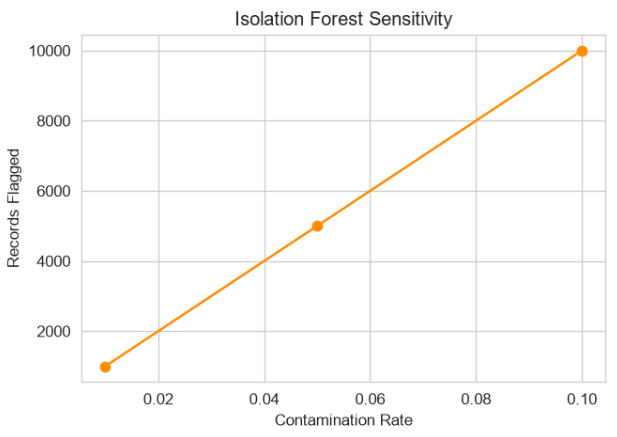
\includegraphics[width=0.85\columnwidth]{mehfo5a.png}\\[2pt]
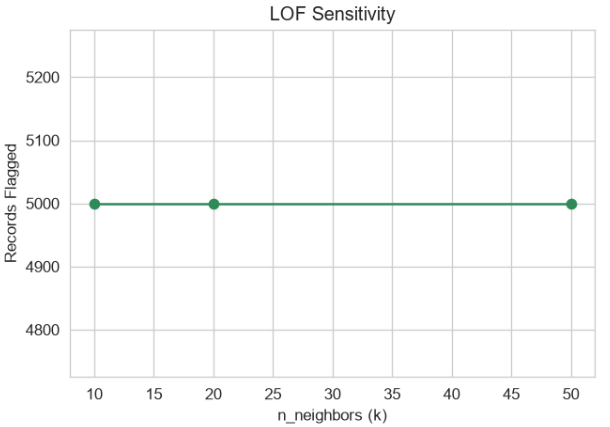
\includegraphics[width=0.85\columnwidth]{mehfo5b.png}
\caption{Flagged-record counts as the Isolation Forest contamination rate (top) and the LOF neighborhood size $k$ (bottom) are varied.}
\label{fig:sens}
\end{figure}

\subsection{Visual comparison}
Figure~\ref{fig:box} shows speed before and after removal by each detector. The raw data contain speeds of several hundred km/h that stretch the axis; after any of the four detectors is applied, the remaining distribution is compact. Figure~\ref{fig:flagpct} repeats the flag rates of Table~\ref{tab:dev} graphically, and Fig.~\ref{fig:scatter-if} shows the trips flagged by Isolation Forest in the distance-speed plane. The flagged trips include the extreme-speed and long-distance points as well as a dense group at short distances, whereas the unflagged trips cluster in a compact region near the origin.

\begin{figure}[!t]
\centering
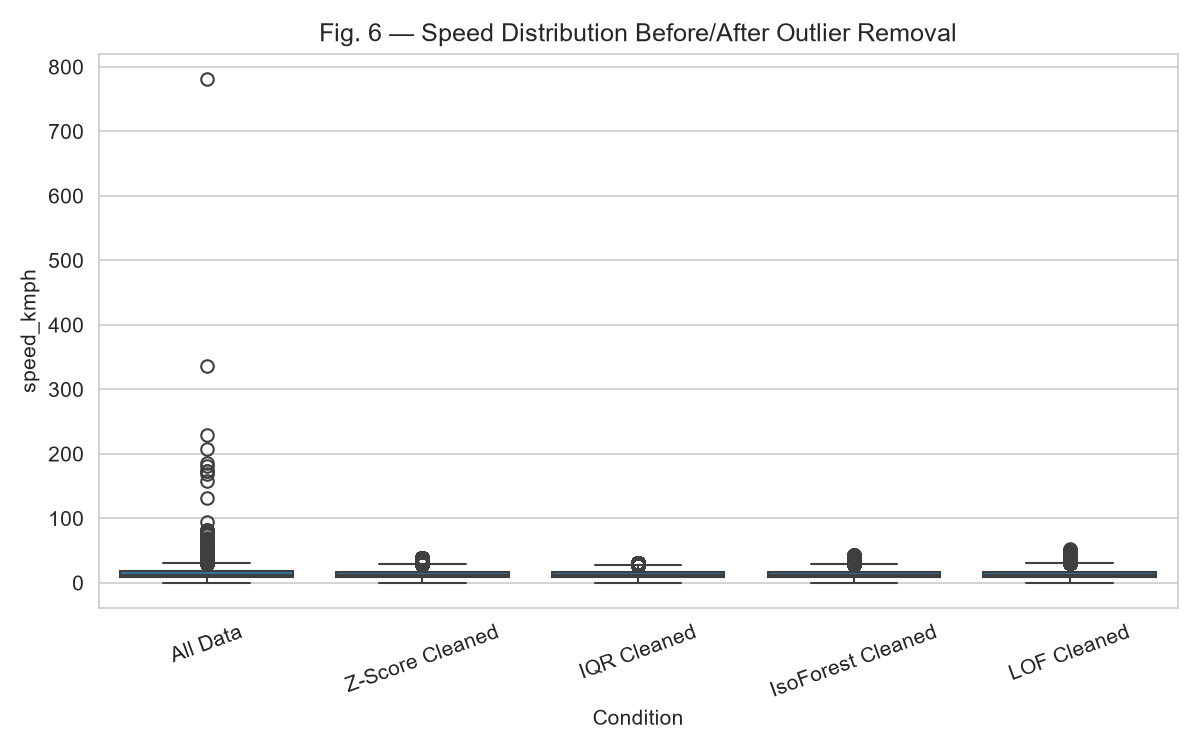
\includegraphics[width=\columnwidth]{mehfo6.png}
\caption{Distribution of trip speed before and after removal of each detector's flagged trips.}
\label{fig:box}
\end{figure}

\begin{figure}[!t]
\centering
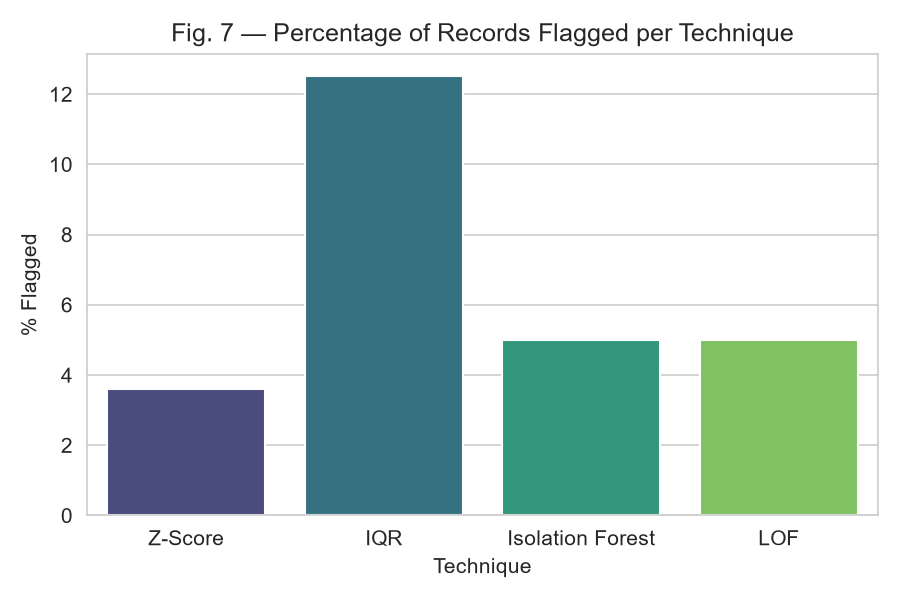
\includegraphics[width=0.85\columnwidth]{mehfo7.png}
\caption{Percentage of trips flagged by each detector (development sample).}
\label{fig:flagpct}
\end{figure}

\begin{figure}[!t]
\centering
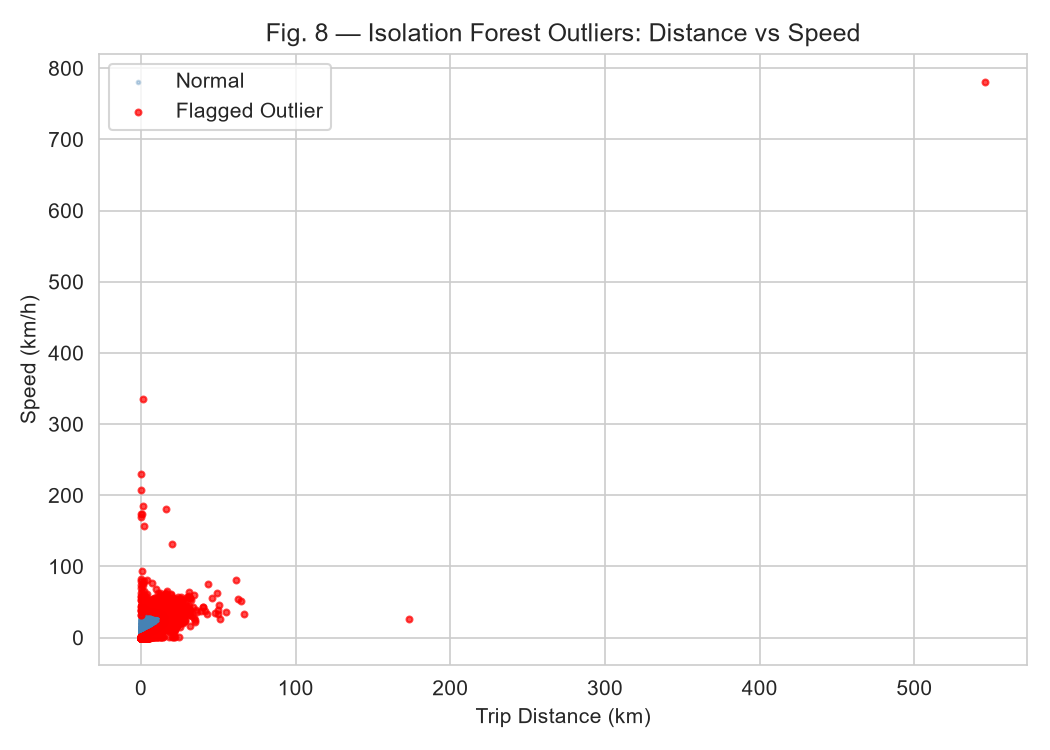
\includegraphics[width=\columnwidth]{mehfo8.png}
\caption{Distance versus speed, with trips flagged by Isolation Forest highlighted.}
\label{fig:scatter-if}
\end{figure}

\subsection{Reproducibility check}
Isolation Forest is randomized, so we repeated it with three seeds (42, 7, and 123). The flagged counts were 4999, 5000, and 5000 (mean 4999.7, standard deviation 0.47), but the count is stable by construction because the contamination parameter fixes it. The informative quantity is whether the same trips are flagged, and Table~\ref{tab:ext_stability} reports the pairwise Jaccard similarity between seeds. The mean Jaccard similarity between seeds is 0.867, so roughly one flagged trip in seven differs from seed to seed. Isolation Forest is far more stable than LOF is with respect to $k$, but it is not deterministic.

\exttable{ext_stability}{Table: stability of flagged sets}

\subsection{Runtime and operating trade-offs}
The runtime differences are large. The Z-score and IQR rules need 0.160~s and 0.200~s on all 1.46 million rows, whereas Isolation Forest needs 18.552~s, about 116 times as long as the Z-score rule. LOF took 1.673~s on its 300,000-row sub-sample, which cannot be compared directly with a full-data run. The cost of LOF depends on neighbor search, which is cheap with a spatial index in three dimensions and expensive in the worst case. For real-time cleaning of incoming trips, a classical rule is the practical first pass, despite IQR's low plausibility precision. Isolation Forest and LOF fit periodic batch jobs. Section~\ref{sec:extended} shows that LOF is cheaper than the sub-sample experiment suggested: on all 1,458,644 trips a kd-tree search finishes in about 22 seconds.

\section{Extended Experiments}
\label{sec:extended}
The experiments in this section address limitations of the base study. All tables are generated by the accompanying script, \texttt{run\_all.py}, and nothing is reported here that the script does not produce.

\subsection{Additional baselines and feature scaling}
The base study ran every detector on raw features. Euclidean distances, and therefore LOF, are sensitive to feature scale: with duration in seconds (standard deviation 5237) alongside distance in kilometers (4.29) and speed in km/h (14.97), neighbor distances are dominated by duration. To test how much this matters, we repeat the comparison in a second feature space, $\log(1+\mathbf{x})$ followed by robust scaling (median and IQR), and we add two baselines that were not in the conference version: the MAD-based modified Z-score with threshold 3.5 \cite{leys2013,iglewicz1993} and the Mahalanobis distance from a minimum covariance determinant fit \cite{rousseeuw1999}, flagged against a $\chi^2_3$ cutoff at the 97.5th percentile. Table~\ref{tab:ext_detectors} reports flag rate, runtime, plausibility precision, and plausibility recall for all six detectors in both spaces.

\exttable{ext_detectors}{Table: six detectors x two feature spaces}

Two results stand out. On raw features, MAD behaves like the IQR rule (11.67\% flagged, 3.8\% recall), because it too has no usable lower boundary, whereas the MCD distance flags 38.1\% of all trips, because a $\chi^2$ cutoff assumes an elliptical distribution that these skewed data do not follow; its 92.9\% recall comes from flagging a large share of the dataset and is accompanied by 1.65\% precision. After logarithmic transformation and robust scaling, the Z-score, IQR, MAD, and Isolation Forest detectors each recover all 676 rule-violating trips, with precision of 36.7\% (Z-score, 1.84\% flagged), 24.3\% (MAD, 2.78\% flagged), 11.9\% (IQR, 5.70\% flagged), and 13.5\% (Isolation Forest, 5.00\% flagged). LOF moves the other way: its recall falls from 56.2\% on raw features to 28.4\%. Euclidean neighbor distances on raw features are dominated by duration, whose standard deviation (5237~s) dwarfs those of distance (4.29~km) and speed (14.97~km/h), which is consistent with LOF's raw-feature advantage coming largely from very short durations. The reference rules also use thresholds on these same variables, so the high recall of the log-scaled global rules partly reflects that overlap, a point we return to in Section~\ref{sec:discussion}.

\subsection{Injected-anomaly benchmark}
Plausibility overlap uses rules that involve the same features the detectors see, which is partly circular. To obtain a label-based comparison, we start from the development-sample trips that satisfy all three plausibility rules, inject 1\% synthetic anomalies, and measure how well each detector's score ranks them. Four anomaly types mimic the faults seen in the raw data: durations shortened to under ten seconds, durations multiplied by 20 to 200 (a meter left running), distances multiplied by 15 to 80 (a GPS jump), and distances set to zero. We report area under the ROC curve, average precision, and precision among the top $k$ scores, where $k$ equals the number of injected anomalies, averaged over random seeds (Table~\ref{tab:ext_injection}). The benchmark is synthetic and so shows what each detector \emph{can} find, not how often real faults take these forms.

\exttable{ext_injection}{Table: AUROC / AP / P@k with injected anomalies}

After logarithmic transformation and robust scaling, the IQR and MAD rules rank the injected anomalies best (AUROC 0.999, average precision 0.919), ahead of the Z-score rule (0.999, 0.895) and Isolation Forest (0.998, 0.769); the MCD distance reaches 0.982 and 0.398. LOF is clearly last (0.666 and 0.103). On raw features most detectors do worse, the exceptions being LOF (AUROC 0.747 and average precision 0.267, against 0.666 and 0.103 after scaling) and the average precision of the MCD distance. The ordering changes somewhat: Isolation Forest has the highest AUROC on raw features (0.981) while the IQR rule keeps the highest average precision (0.654), and LOF remains last on both measures (0.747 and 0.267). Because the injected anomalies are large departures from the bulk of the data, global detectors are favored by construction, so this benchmark should be read as showing what each detector can find, not as a verdict on LOF in settings where anomalies are local.

\subsection{Downstream regression on a common evaluation set}
To make the five regression conditions comparable, every detector's cleaned training set is evaluated on the same held-out partition, both as it stands and after removing the rule-violating trips. We report RMSE together with MAE, median absolute error, and RMSLE, because RMSE alone is dominated by a few extreme targets, and we repeat the split over several random seeds to give a spread (Table~\ref{tab:ext_downstream}).

\exttable{ext_downstream}{Table: downstream errors on common test sets, mean +- std}

The interpretation of this table is given in Section~\ref{sec:results}: squared error does not move, whereas absolute errors fall by 6 to 13\% (mean) and 15 to 37\% (median) in the raw feature space. Feature scaling changes the detectors' effect on these measures only slightly.

\subsection{LOF on the complete dataset}
The conference version restricted LOF to 300,000 rows on the grounds that neighbor search scales quadratically. That concern does not apply in three dimensions with a kd-tree: LOF ran on all 1,458,644 trips in 22.3 s on raw features and 21.3 s after scaling, on a single processor core (Table~\ref{tab:ext_fulllof}). This removes the sample-size caveat attached to Table~\ref{tab:full}. Against the rule-based reference set computed on the full data (9,293 trips, 0.64\%), LOF's precision is 2.95\% and its recall 23.2\% on raw features, lower than on the development sample because 5\% of 1.46 million trips is a much larger flagged set relative to the reference set.

\exttable{ext_fulllof}{Table: full-data LOF}

\subsection{Two-stage pipelines}
The complementary behavior of the detectors suggests combining them: a fast global rule or Isolation Forest removes gross errors, and LOF is then run on the remaining trips to catch small-value and local anomalies. Table~\ref{tab:ext_twostage} compares these pipelines with their single-detector components against the plausibility reference set. Because the second stage flags a fixed 5\% of what remains, the combined flag rate necessarily exceeds either stage alone, so precision should be read together with the flag rate.

\exttable{ext_twostage}{Table: two-stage pipelines}

Adding LOF as a second stage after Isolation Forest raises recall from 29.9\% to 45.3\%, but it nearly doubles the flag rate (5.00\% to 9.75\%) and lowers precision from 4.04\% to 3.14\%. After the IQR rule the second stage lifts recall from 4.1\% to 32.8\% at 16.9\% flagged. None of these pipelines reaches the 56.2\% recall that LOF achieves alone on raw features at 5\% flagged (Table~\ref{tab:plaus}), so in our tests the two-stage design is not an improvement; the extra trips recovered mostly reflect the larger number flagged.

\section{Discussion}
\label{sec:discussion}

\subsection{Why the criteria disagree}
The criteria measure different things. Plausibility asks whether flagged trips break a physical rule, and it rewards detectors that look at both tails of a variable. Agreement asks whether two detectors would produce the same cleaned dataset. Downstream effect asks whether removing the flagged trips changes a model's error on a fixed evaluation set, and under squared error it is dominated by the few largest values. Our results already show that the first two can diverge sharply: LOF finds the sparse small-value records that the rules define as implausible, which the upper-fence rules cannot reach by construction, yet it overlaps little with any other detector. The corrected downstream results fit this picture. LOF, which recovers the most rule-violating trips on raw features, gives the smallest reduction in absolute error among the four detectors, whereas the global detectors, which remove the extreme long and fast trips, give larger reductions. A plausible reading is that the rule-violating trips are few (0.68\% of the sample) and mostly short, and a linear model driven by distance is hardly affected by them, whereas the extreme long-duration records pull its coefficients. We have not tested this explanation directly. This is why we do not collapse the criteria into a single ranking.

\subsection{Choosing a detector}
Table~\ref{tab:guidance} summarizes the guidance that follows from the results. A two-stage pipeline follows naturally from the complementary behavior observed here, and Table~\ref{tab:ext_twostage} tests it directly. It does not support the combination: the second stage raises recall mainly by flagging more trips, and no pipeline beats LOF alone on raw features.

\begin{table}[!t]
\caption{Guidance on detector choice under different operating constraints, derived from the results.}
\label{tab:guidance}
\centering
\small
\begin{tabular}{p{0.28\columnwidth}p{0.3\columnwidth}p{0.3\columnwidth}}
\hline
Constraint & Suitable detector & Reason \\
\hline
Real-time, full data & IQR or Z-score & Sub-second on 1.46 M rows \\
Minimize downstream absolute error & Isolation Forest, Z-score, or IQR & Largest MAE reductions, within noise of each other \\
Find physically implausible trips & Z-score or MAD on log-scaled features; LOF on raw features & 100\% recall (log, global rules); 56\% recall (raw LOF) \\
Periodic batch audit & Isolation Forest, LOF & Higher cost acceptable \\
\hline
\end{tabular}
\end{table}

\subsection{Threats to validity}
Several limitations frame these results.

\emph{No ground truth.} All five criteria are proxies. The injected-anomaly benchmark in Section~\ref{sec:extended} partly addresses this, but its anomaly types are our own assumptions.

\emph{Partly circular reference set.} The plausibility rules are expressed in terms of the same duration, distance, and speed that the detectors consume. A detector that thresholds those variables can match them for that reason alone. The rules were written by us, not drawn from an independent standard, and their thresholds, though reasoned, are arbitrary.

\emph{Fixed contamination.} Isolation Forest and LOF flag exactly 5\% by construction. The 5\% figure is deliberately larger than the 0.68\% rule-violation rate, and any conclusion comparing flag rates between these two detectors and the classical rules reflects the parameter, not the data. No grid search was run, because without labels there is no objective on which to select an optimum; the sensitivity analysis characterizes the response instead.

\emph{Significance.} We have not applied null-hypothesis tests. With a million records almost any difference is statistically significant, so the effect sizes, such as the nearly twofold gap in plausibility precision between LOF and Isolation Forest or the several-fold gap in recall between LOF and the classical rules, are the more relevant evidence. The repeated-split spreads in Section~\ref{sec:extended} add a measure of variability.

\emph{Earlier protocol.} The conference version's downstream experiment cleaned the whole sample before splitting, so each detector was scored on a different filtered test set. We have replaced it, and conclusions about downstream effect rest only on the corrected protocol.

\emph{Dependence on feature scale.} The ordering of detectors on the plausibility criterion reverses between raw and log-scaled features, so no ranking should be quoted without naming the feature space. We did not tune scaling beyond the single log-plus-robust transformation.

\emph{Single dataset.} All results come from one year of New York yellow-cab data. Other cities, fleets, or years may differ in error rates and distributions, and the ranking of detectors may change with them.

\section{Conclusion}
\label{sec:conclusion}
We compared the Z-score rule, Tukey's IQR fences, Isolation Forest, and LOF as record-level cleaners for 1,458,644 New York taxi trips, using a label-free protocol built from flag rate, pairwise agreement, plausibility overlap, runtime, and downstream regression error. The IQR rule flagged the most trips (12.51\%) and the Z-score rule the fewest (2.92\%), a gap explained by how heavily the mean and standard deviation are inflated by the skewed tail. Agreement between detectors was low, except between Isolation Forest and the Z-score rule (Jaccard 0.697).

The clearest result is that conclusions about detector quality depend on the feature space. On raw features, upper-fence rules cannot flag implausibly small values, because their lower boundaries are negative, and LOF recovered 56\% of the physically implausible trips against 2.5\% and 4.1\% for the Z-score and IQR rules. After logarithmic transformation and robust scaling the picture reverses: the Z-score, IQR, MAD, and Isolation Forest detectors recovered every such trip, and LOF recovered 28\%. On injected anomalies with known labels, the IQR and MAD rules ranked best after scaling, and LOF ranked worst in both spaces. Agreement between detectors was low, and LOF's flagged set changed considerably with the neighborhood size (Jaccard as low as 0.24).

Our earlier downstream result, a large RMSE reduction from IQR cleaning, came from cleaning the test set along with the training set. Under a corrected protocol with a common test set, squared error did not change, and mean absolute error fell by 6 to 13\%, with the three global detectors close together and LOF improving least.

For practitioners the guidance is to state the feature space, to log-transform skewed positive variables before applying global rules, and to treat LOF as a complement rather than a replacement. LOF is also practical at full scale (about 22 seconds for 1.46 million trips on one core). A two-stage pipeline did not outperform LOF alone in our tests. Future work includes evaluating other cities and years, using independent ground truth where it exists, and tuning the feature transformation.

\section*{Data Availability}
The dataset is publicly available from Kaggle \cite{tlc2016}. \todo{Add the repository URL (GitHub/Zenodo) containing the code, \texttt{extended\_experiments.py}, and the random seeds.}

\section*{Acknowledgment}
\todo{Acknowledge funding, supervisors, or institutional support. If generative AI tools were used in preparing the manuscript text, IEEE's author policy requires disclosing this here; check the current IEEE Access author guidelines for the exact wording.}

\bibliographystyle{IEEEtran}
\bibliography{refs}

\begin{IEEEbiographynophoto}{Mehfooza M}
\todo{Add biography: degrees, current position at VIT Vellore, research interests.}
\end{IEEEbiographynophoto}

\begin{IEEEbiographynophoto}{Likith Pulivarthi}
\todo{Add biography.}
\end{IEEEbiographynophoto}

\begin{IEEEbiographynophoto}{Rana Yash Raj Pratap Singh}
\todo{Add biography.}
\end{IEEEbiographynophoto}

\begin{IEEEbiographynophoto}{Vinayak Raj}
\todo{Add biography.}
\end{IEEEbiographynophoto}

\EOD

\end{document}
